\chapter{Evaluation}
\label{chap:eval}

In this chapter, the evaluation result of the current work is presented after running experiment feature of RUMIS. We focus on testing the quality of rule revisions in terms of conviction measure, and how precise are their predictions. The chapter is organized as follows, first, the setting of the experiment is discussed. Second, the quality of rulesets and their predicted facts are assessed. Finally, we present the runtime performance of RUMIS with different datasets.

\section{Setting}

\textbf{Dataset.} To measure the quality of rules and their predictions, the occurrence of ideal graph $\cG^i$, i.e. the ideal KG containing all true facts from real world, is necessary. Nonetheless, achieving $\cG^i$ is infeasible and impracticable. Hence, some KG $\cG^i_{\mi{appr}}$ with a large number of true facts can be exploited as an approximated version for $\cG^i$. Besides, the learning KG $\cG$ is created by deleting 20\% of the triples over every binary relation, and retaining all unary facts in $\cG^i_{\mi{appr}}$. It is guaranteed that there is no isolated vertex, i.e the node which does not connect to any other nodes in $\cG$. In our experiment, YAGO3~\cite{ref28}, part of Wikidata~\footnote{\url{https://www.wikidata.org}} and IMDB~\footnote{\url{http://people.mpi-inf.mpg.de/~gadelrab/downloads/ILP2016}} datasets are used as the ideal KGs. YAGO3 covers a variety of domains and contains roughly 1.8 million entities, 38 predicates, and 20.7 million triples. Meanwhile, IMDB only focus on movie content collected from the IMDB website~\footnote{\url{http://imdb.com}}, there are 112 thousand entities, 38 predicates and 583 thousand triples in this KG.

Besides, 1 million facts with 238 thousand entities and 443 predicates are sampled from Wikidata for the approximated ideal KG by the following way. In details, thanks to randomly choosing facts in the format \textit{$<$subject$>$ $<$memberOf$>$ $<$object$>$} where \textit{$<$object$>$} is in the list of manually chosen popular football clubs, famous footballers and coaches (seeding set) are sampled from Wikidata. After that, all the entities that can be visited from any node in the seeding set (chosen entities) are collected for the ideal KG. These chosen entities and all possible links between them in the original Wikidata are sampled for the smaller scale. This new KG is expected to have specific domain where facts are related to football and sports.

Figure~\ref{fig:venn} indicates the ideal, approximated and available KGs used in the current work. Besides, the extension KGs $\cG_{\cR_{\mi{H}}}$, $\cG_{\cR_{\mi{NM}}}$ obtained by resp. applying $\cR_H$ and its revision $\cR_{NM}$ to $\cG$ can be seen in the figure. The RUMIS aims to tackle the KG completion problem by narrowing the difference between the $\cG_{\cR_{\mi{NM}}}$ and $ \cG^i$.

\begin{figure}[ht]
\centering
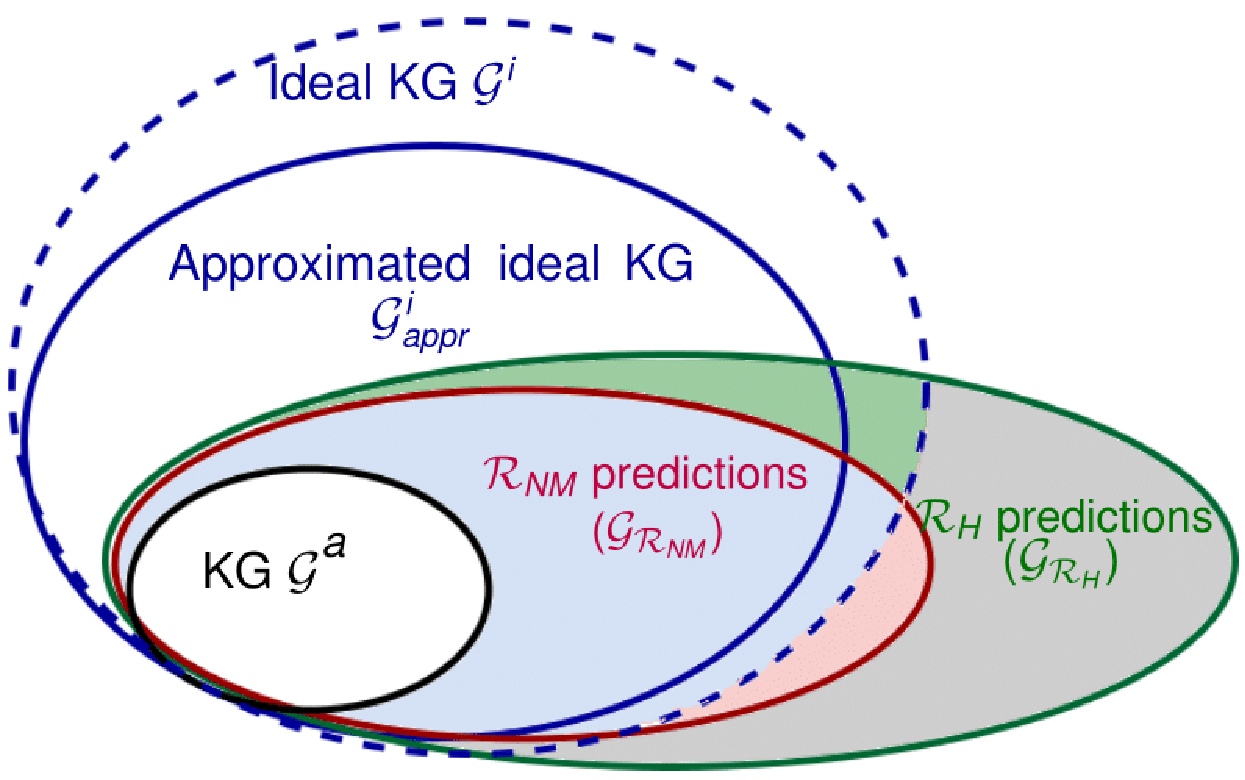
\includegraphics[width=0.45\textwidth]{figures/big_pic_exp}
\caption{The Ideal, Available and Extended KGs.}
\label{fig:venn}
\end{figure}

\textbf{Setup.} In our experiment, RUMIS is executed on a server which has Linux OS, 40 cores and 400GB RAM memory. As the data preparation, positive rules with the format \textit{h(X, Z) $\leftarrow$ p(X, Y), q(Y, Z)} are explored from $\cG$ and ranked according to the \textit{absolute support} measure. The positive rule mining function of RUMIS (Chapter~\ref{chap:system}) is exploited in this step. After that, the positive rules are revised with the methodology presented in the Chapter~\ref{chap:frame}, here \textit{conviction} is used for the $\mi{rm}$ rule measure. More specifically, exceptions for each positive rule are ranked and the optimal one in terms of conviction score is added to the final set. This ranking feature of RUMIS is applied for different strategies such as \emph{Naive}, \emph{PM}, and \emph{OPM}, and the results are stored in $\mi{\cR_{N}}$, $\mi{\cR_{PM}}$, and $\mi{\cR_{OPM}}$, resp.

\section{Ruleset Quality}

For every row in the Table~\ref{tab:rules_quality}, we fix the top-$\mi{k}$ ($k=5,30,$ ... $100$) positive rules $\cR_{H}$ from the preparation step. Then the \textit{average conviction} of the rules and their revisions are found for YAGO and IMDB by using RUMIS. It can be seen that the quality of the positive rulesets is always improved in terms of the average conviction thanks to the revision process. Besides, in general while the average quality of every column has a decreasing trend with the appearance of rules having lower precision levels, the enhancement ratio between positive rules and their revisions steps up and reaches the peak of $10\%$ for top-60 Wikidata rules. That means with low quality Horn rules, the introduction of negated atoms significantly boost up their precision.

\begin{table}[ht]
\centering
\footnotesize
\renewcommand*{\arraystretch}{1.07}
\centering



\footnotesize{
\resizebox{\columnwidth}{!}{%

\begin{tabular}{|l|llll|llll|llll|}
\hline
       \multirow{2}{*}{\textbf{\textit{topk}}}                    & \multicolumn{4}{c|}{\textbf{YAGO}}        & \multicolumn{4}{c|}{\textbf{IMDB}}  & \multicolumn{4}{c|}{\textbf{Sample WIKIDATA}}      \\ \cline{2-13} 
       %\hline
 & $\cR_{H}$ & $\cR_{N}$ & $\cR_{PM}$ & $\cR_{OPM}$ & $\cR_{H}$ & $\cR_{N}$ & $\cR_{PM}$ & $\cR_{OPM}$ & $\cR_{H}$ & $\cR_{N}$ & $\cR_{PM}$ & $\cR_{OPM}$ \\ \hline
5   & 1.3784 & 1.3821 & 1.3821 & 1.3821 & 2.2670 & 2.3014 & 2.3008 & 2.3014 & 3.2282 & 3.2342 & 3.2340 & 3.2342\\ %\hline
30   & 1.1207 & 1.1253 & 1.1236 & 1.1237 & 1.5453 & 1.5644 & 1.5543 & 1.5640 & 3.1118 & 3.4315 & 3.4194 & 3.4271\\ %\hline
50   & 1.0884 & 1.0923 & 1.0909 & 1.0913 & 1.3571 & 1.3749 & 1.3666 & 1.3746  & 2.7115 & 2.9193 & 2.9070 & 2.9135\\ %\hline
60   & 1.0797 & 1.0837 & 1.0823 & 1.0829 & 1.3063 & 1.3221 & 1.3143 & 1.3219  & 2.4930 & 2.7101 & 2.6986 & \textbf{2.7046}\\ %\hline
70   & 1.0714 & 1.0755 & 1.0736 & 1.0744 & 1.2675 & 1.2817 & 1.2746 & 1.2814  & 2.3395 & 2.5272 & 2.3931 & 2.5219\\ %\hline
80   & 1.0685 & 1.0731 & 1.0710 & 1.0720 & 1.2368 & 1.2499 & 1.2431 & 1.2497  & 2.4071 & 2.5781 & 2.4597 & 2.5734\\ %\hline
100   & 1.0618 & 1.0668 & 1.0648 & 1.0659 & 1.3074 & 1.4100 & 1.3987 & 1.4098  & 2.3258 & 2.4847 & 2.3859 & 2.4806\\ \hline

\end{tabular}

}
}

% \centering
% \caption{My caption}
% \label{my-label}
% \begin{tabular}{l|l|l|l|l|l|l|l|l|}
% \cline{2-9}
%                            & \multicolumn{4}{c|}{YAGO manual}        & \multicolumn{4}{c|}{IMDB top rules}        \\ \hline
% \multicolumn{1}{|l|}{\textit{topk}} & $\cR_{H}$ & $\cR_{N}$ & $\cR_{PM}$ & $\cR_{OPM}$ & $\cR_{H}$ & $\cR_{N}$ & $\cR_{PM}$ & $\cR_{OPM}$ \\ \hline
% \multicolumn{1}{|l|}{5}    &   1.10    &   1.11    &    1.20    &    1.15     &   2.27    &   2.3    &   2.89     &  2.55       \\ \hline
% \multicolumn{1}{|l|}{10}   &    1.10   &   1.11    &    1.23    &    1.18     &   1.9    &   1.92    &    4.74    &  2.07       \\ \hline
% \multicolumn{1}{|l|}{15}   &   1.12    &   1.13    &    1.32    &    1.18     &   1.8    &   1.82    &   5.25     &   1.98      \\ \hline
% \multicolumn{1}{|l|}{20}   &       &       &        &         &       &       &        &         \\ \hline
% \end{tabular}

\smallskip
\caption{The Average Quality of the Top Positive and Nonmonotonic Rules.}
\label{tab:rules_quality}
%\vspace*{-1.7\baselineskip}
\end{table}

\section{Prediction Quality}

Among top-50 (for IMDB, YAGO3) and top-300 (for Wikidata) of positive rules mined in the preparation step, 5 of them are sampled as $\cR_H$ and then the methodology is applied to the datasets. After that, the predictions of the $\cR_H$ and their revisions are analyzed to evaluate the proposed theory.

To this end, these rulesets are applied to the learning KG $\cG$ using DLV tool~\cite{dlv}. Subsequently, we achieve $\cG_{\cR_\mi{H}}$, $\cG_{\cR_\mi{N}}$, $\cG_{\cR_\mi{PM}}$ and $\cG_{\cR_\mi{OPM}}$ for $\cR_H$ and their revisions, resp. Some statistics for that is shown on Table~\ref{tab:prediction_res} where the first three columns indicate head relations in the $\cR_H$, the
quantity of new predictions, i.e. predicted facts not included in $\cG$ and the part of these predictions which are outside $\cG^i_{\mi{appr}}$. The statistics in the second and third columns is available for all ranking options.

\begin{table}[ht]
\centering

% \begin{tabular}{c|l|llll|llll}
% \hline
%  \multirow{2}{*}{}              &   \multirow{2}{*}{\textbf{$\mi{head(r)}$}}   	& \multicolumn{4}{c|}{\textbf{predictions}} 						&  \multicolumn{4}{c}{\textbf{outside $\cG^i_{appr}$}}  				\\ \cline{3-10} 
%          						&  									& $\cR_\mi{H}$  & $\cR_{N}$ & $\cR_{PM}$  		& $\cR_{OPM}$ &  $\cR_\mi{H}$     & $\cR_{\mi{N}}$ 	& $\cR_\mi{PM}$     & $\cR_{\mi{OPM}}$    \\ \hline
% %\multirow{4}{*}{\rotatebox{90}{YAGO}}
% & directed & 41079 & 39174 & 39174 & 39174  & 41021 & 39116 & 39116 & 39116 \\ %\cline{2-10}
%  & gradFrom & 3519 & 3456 & 3456 & 3456  & 3363 & 3300 & 3300 & 3300 \\ %\cline{2-10}
%  & citizenOf & 3407 & 2883 & 2883 & 2883  & 3360 & 2836 & 2836 & 2836 \\ %\cline{2-10}
%  & bornIn & 110283 & 108317 & 109846 & 108317 & 109572 & 107607 & 109137 & 107607 \\ \hline\hline %\cline{1-10}
% %\multirow{4}{*}{\rotatebox{90}{IMDB}} 
% & actIn & 1231 & 1214 & 1230 & 1214 & 1148 & 1131 & 1147 & 1131 \\ %\cline{2-10}
%  & genre & 629 & 609 & 618 & 609  & 493 & 477 & 482 & 477 \\% \cline{2-10}
%  & hasLang & 173 & 102 & 125 & 102 & 163 & 92 & 115 & 92 \\ %\cline{2-10}
%  & prodIn & 2489 & 2256 & 2327 & 2327 & 2488 & 2255 & 2326 & 2326 \\ \cline{1-10}
% \end{tabular}
\footnotesize{
\resizebox{\columnwidth}{!}}}  				\\ \cline{2-12} 
 		& $\cR_\mi{H}$  & $\cR_{\mi{N}}$ & $\cR_{\mi{PM}}$  		& $\cR_{\mi{OPM}}$ &  $\cR_\mi{H}$     & $\cR_{\mi{N}}$ 	& $\cR_\mi{PM}$     & $\cR_{\mi{OPM}}$  & $\cR_{\mi{N}}$ 	& $\cR_\mi{PM}$     & $\cR_{\mi{OPM}}$   \\ \hline

%\multirow{4}{*}{\rotatebox{90}{IMDB}} 
 $\mi{{I}{:}{actedIn}}$ & 1231 & 1214 & 1230 & 1214 & 1148 & 1131 & 1147 & 1131 &90 & 100 & 90\\ %\cline{2-10}
 $\mi{{I}{:}{genre}}$ & 629 & 609 & 618 & 609  & 493 & 477 & 482 & 477 &50 & 20 & 50\\% \cline{2-10}
 $\mi{{I}{:}{hasLang}}$ & 173 & 102 & 125 & 102 & 163 & 92 & 115 & 92 &  60 & 100 & 60\\ %\cline{2-10}
 $\mi{{I}{:}{prodIn}}$ & 2489 & 2256 & 2327 & 2327 & 2488 & 2255 & 2326 & 2326 & 10 & 10 & 30 \\ \cline{10-12}
 &  &  &  &  &  &  &  &  	& 52.50  & 45.16   & \textbf{57.75}  \\
\hline 
$\mi{{Y}{:}{direct}}$ & 41079 & 39174 & 39174 & 39174  & 41021 & 39116 & 39116 & 39116 & 100 & 100 & 100   \\
 $\mi{{Y}{:}{grFrom}}$ & 3519 & 3456 & 3456 & 3456  & 3363 & 3300 & 3300 & 3300 & 100 & 100 & 70 \\ 
 $\mi{{Y}{:}{citizOf}}$ & 3407 & 2883 & 2883 & 2883  & 3360 & 2836 & 2836 & 2836 & 50 & 50 & 70 \\ 
 $\mi{{Y}{:}{bornIn}}$ & 110283 & 108317 & 109846 & 108317 & 109572 & 107607 & 109137 & 107607 &90& 90 & 100 \\ \cline{10-12}  
 &  &  &  &  &  &  &  &  	& 85  & 85   & 85 \\
 \hline 
 \end{tabular}}}

\smallskip
\caption{New Facts Predicted by the Rulesets for IMDB (\textit{I}) and YAGO (\textit{Y}).}
\label{tab:prediction_res}
%\vspace*{-1.7\baselineskip}
\end{table}

It can be inferred that there are not many predicted facts included in $\cG^i_{\mi{appr}}$ ($\approx$9\% in IMDB and $\approx$2\% in YAGO ideal KGs). This illustrates our expectation since the latter is a general purpose KG and it misses a lot of facts. Also, it is crucial to see that the sampled Horn rules and their revisions generate approximately the same quantity of correctly predicted facts which are confirmed in $\cG^i_{\mi{appr}}$. E.g., in YAGO $\cG_{\mi{\cR_H}}\backslash \cG_{\mi{\cR_{PM}}} \cap \cG^i_{\mi{appr}}=\emptyset$ holds true, that means the green region has nothing in common with the approximated ideal KG in Figure~\ref{fig:venn}. In other words, the appearance of exceptions does not remove any correct facts predicted by $\cR_H$ according to $\cG^i_{\mi{appr}}$.

To guarantee the fairness of the comparison between predictions generated by different rulesets, it is necessary to keep the $\cR_H$ not totally false. Because once the sampled positive rules always generate incorrect facts, inserting arbitrary negated atoms may filter out some incorrect ones, followed by the enhancement of the revision precision. Besides, the numbers in the third column of Table~\ref{tab:prediction_res} according to $\cR_H$ are big, that means there are a lot of facts generated by this ruleset outsite the approximated ideal KG, and no ground truth is available to verify them. Thus, we have to manually check the generated facts using the Internet resource. Since the quantity of them is huge, we propose to randomly select maximum 20 new predictions for each head predicate in $\cR_H$. With the selected IMDB facts, the accuracy is 70\% while this number of YAGO and Wikidata datasets are 30\% and 55\%, resp. It can be inferred that the quality of mined positive rules is not totally false and fulfills the above requirement.

Since the size of difference sets between KGs extended by applying $\cR_H$ and its revisions to $\cG$ is also huge, we have to apply the sampling again. Here for each head relation from the difference sets $\cG_{\cR_\mi{H}}\backslash \cG_{\cR_{\mi{N}}}$, $\cG_{\cR_\mi{H}}\backslash \cG_{\cR_{\mi{PM}}}$ and $\cG_{\cR_\mi{H}}\backslash \cG_{\cR_{\mi{OPM}}}$, 10 facts are randomly sampled for manual check. In the last column of the Table~\ref{tab:prediction_res}, the proportion of false facts in the difference sets are presented. These facts are called ``correctly removed" and correspond to the grey region in in Figure~\ref{fig:venn}. With IMDB dataset, among all the strategies, OPM ranking is always the best one with 57.75\% and 97.5\% correctly removed predictions for IMDB and Wikidata, resp. Meanwhile, all the rankers share the same quality of 85\% correctly removed facts in YAGO. Because the predictive power of the rules in IMDB is better than those in YAGO, the revisions of the latter play a higher impact than the former.

\section{Running Times}

RUMIS mines 100 positive rules and their $\mi{EWS}$s from IMDB and YAGO in 7 and 68 seconds, resp. The mean number of exceptions for each positive rule is 1600 for the former and 10900 for the latter. With IMDB, the exceptions for Naive, PM and OPM strategies are ranked within 9, 62 and 24 seconds, resp. Meanwhile in YAGO, these numbers are 45, 177 and 112 seconds with the same ranking function. As regards the step of applying final revisions to the KG $\cG$, the DLV tool finishes after 8 and 310 seconds with IMDB and YAGO, resp.

\begin{figure}[t]
    \centering
   
    \vspace{-.2cm}
    \begin{tabular}{l}
 {\scriptsize
        $\mi{r_1: writtenBy(X, Z)}  \leftarrow
        \mi{hasPredecessor(X, Y)},\mi{writtenBy(Y, Z)},$ $ \textbf{not}$  $\mi{american\_film(X)} $}\\        
       {\scriptsize 
$\mi{r_2:  actedIn(X, Z)}  \leftarrow
        \mi{isMarriedTo(X, Y)},\mi{directed(Y, Z)},$ $ \textbf{not}$  $\mi{silent\_film\_actor(X)} $} \\
          {\scriptsize 
$\mi{r_3:  isPoliticianOf(X, Z)}  \leftarrow
        \mi{hasChild(X, Y)}{,}\mi{isPoliticianOf(Y, Z)}{,}$$ \textbf{not}$  $\mi{vicepresidentOfMexico(X)} $} \\
 \end{tabular}            
    \caption{Examples of the Revised Rules}
 \label{fig:examplerules}
 \vspace{-.4cm}
\end{figure}

\textbf{Example rules.} Some interesting examples of the final revisions are presented in the Figure~\ref{fig:examplerules}. Here 
the $\mi{r_1}$ mined from IMDB dataset indicates that normally movies in the same series share the same writer except the American ones. In addition, $\mi{r_3}$ generated from YAGO reveals an interesting story about politics. To be specific, typically  the pattern that fathers and sons are politicians in the same country is popular, but this does not hold true with Mexican vice-presidents.